\documentclass{article}
\usepackage{graphicx}
\graphicspath{ {images/} }

\title{
    Software Requirements Specification\\
    \begin{large}
        \textit{Golf Course Mapper}
    \end{large}
}
\date{
    \begin{small}
        \today
    \end{small}
}
\author{
    Team Recursive Recursion
}

\begin{document}
    \pagenumbering{gobble}
    \maketitle
    \newpage

    \pagenumbering{arabic}
    \section{Introduction}

    \subsection{Purpose}

    \paragraph{}
    This Software Requirements Specification (henceforth SRS) is intended to be
    a guide on the path of system development. It will aid the developers by
    providing a layout of the project requirements.

    \subsection{Scope}

    \paragraph{}
    The Golf Course Mapper will allow golf course managers to draw the shape of
    their courses using a web application. The owners will map out the details
    of the golf course. This includes mapping the layout of the fairway, green,
    sand and water hazards and details such as the position of the hole and the
    teeing grounds.

    \paragraph{}
    Players currently on the course will then be able to use the provided mobile
    application to view the map of the course and where they are on it
    currently. This has the benefit of allowing players to plan their shots more
    strategically.

    \paragraph{}
    The Golf Course Mapper is not a coaching tool and does not provide a channel
    of communication between the mapper and the player. The web application is
    not to be used by coaches, but solely by managers that wish to map out the
    details of their courses. The Golf Course Mapper is also not a social media
    platform for golfers and will not allow direct communication between
    players.

    \subsection{Definitions, Acronyms \& Abbreviations}
    \begin{itemize}
        \item
            System: Henceforth used to refer to the Golf Course Mapper system
            as a whole.
        \item
            Manager: The manager or owner of a golf course, henceforth used to
            refer to the user of the website.
        \item
            Player: A golf player, henceforth used to refer to the users of the
            mobile application.
        \item
            Website: A web application that is used by golf course managers
            to draw the layout of their golf courses.
        \item
            Mobile App: A native Android mobile app that golf players can use to
            view the golf course.
        \item
            Polygon: The shape drawn on the website to represent a feature of
            the golf course such as the green or the fairway.
        \item
            Back End: The server side that consists of both the DBMS and the
            API.
        \item
            DBMS: Database Management System.
        \item
            API: Application Programming Interface.
    \end{itemize}

    \subsection{Domain Model}

    \paragraph{}
    Refer to figure \ref{domainmodel}, which represents the domain model of the system. At
    the core of the domain model is the \textit{Golf Course} which represents a
    single area where \textit{Players} can go to play the game of golf. Each
    Player is associated with a single Golf Course on which the Player is
    currently playing. Each Golf Course has an assigned \textit{Manager} that is
    solely responsible for mapping and managing the information of the Golf
    Course. Note that a Manager can be assigned to more than one Golf Course.

    \paragraph{}
    Each Golf Course has one or more \textit{Holes} associated with it. A Hole
    represents a single playable map with different \textit{Elements} of spatial
    information. The Elements can be of two different types: \textit{Point}
    Elements and \textit{Polygon} Elements. A Point Element represents
    single-point information of a Hole such as the teeing grounds, location of
    the hole and other points of interest. Polygon Elements represent area
    information of a Hole, such as the area of the rough, fairway, green and
    water and sand hazards.

    \paragraph{}
    A Golf Course may also optionally have Elements that are not associated with
    a specific Hole. This allows the specification of Elements such as points of
    interest or hazardous areas such as bodies of water that may be important to
    more than one Hole. It therefore does not make sense to associate these
    Elements with a specific Hole, but rather with the Golf Course as a whole.
    
    \begin{figure}[h]
    	\centering
    	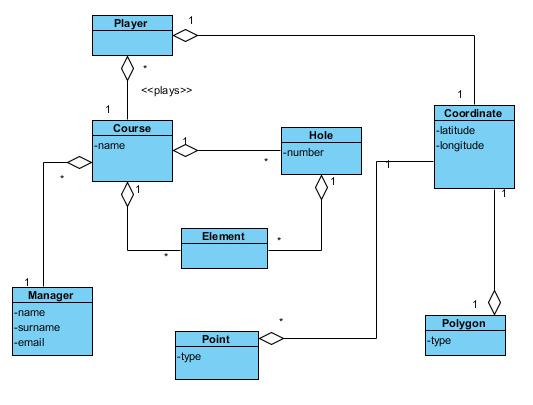
\includegraphics[scale=1]{DomainModel}
    	\caption{Domain model}
    	\label{domainmodel}
    \end{figure}

    \newpage

    \section{Overall Description} 

    \subsection{Product Perspective}

    The product has two user interfaces namely the website and the mobile
    application.\\ The Map that is displayed on the both the website and the
    mobile application is created using the Google Maps API. A custom API was
    created to make database manipulation easier.\\ The mobile application is
    light weight on processing and memory usage since it is only used to view
    the map and do minor calculations such as distance calculation.

    \subsection{Product Functions}
    The main functions are
    \begin{enumerate}
        \item
            Drawing polygons on a map to represent a golf course
        \item
            Displaying the map with the polygons on a mobile device used by
            golfers.
        \item
            Calculate the distance between the player and the hole as well as
            indicating hazards or  obstacles between the player and the hole.
    \end{enumerate}

    \subsection{User Characteristics}
    The product is very simple to use for anyone that has ever had any
    experience working with Google Maps.\\ All icons and user interfaces are
    designed to be as intuitive as possible. This removes the need of a detailed
    tutorial on how to use the system.

    \subsection{Constraints}
    Using a DBMS that simplifies the use of Geographical objects greatly
    improves the development time but it restricts the choice of DBMSs\\ The
    Google Maps API offers 25000 free map loads. After that limit is reached an
    additional fee will be charged for every 1000 loads over the limit.

    \newpage

    \section{Specific Requirements}

    \subsection{Functional Requirements}
    The functional requirements describes the functionality that the System provides. It is drawn from user stories that is also, for simplicity's sake, modelled in figure \ref{fig:usecase1}.
    \begin{itemize}
        \item
            The Manager will register to the Website.
        \item
            The registered Manager will log into the Website.
        \item
            The Manager will create Golf courses.
        \item
            The Manager will add polygons to the course.
        \item
            The Manager will load previously created courses.
        \item
            The Manager will edit courses by drawing extra polygons or removing existing ones.
        \item
        	The Manager will view the map.
        \item
            The Player will view the map on the Mobile App.
        \item
            The Player will select a course of interest  from a list of existing courses.
        \item
            The Player will view the selected course.
        \item
        	The Player will view his position on the map.
    \end{itemize}
    
    \begin{figure}[h]
    \centering
    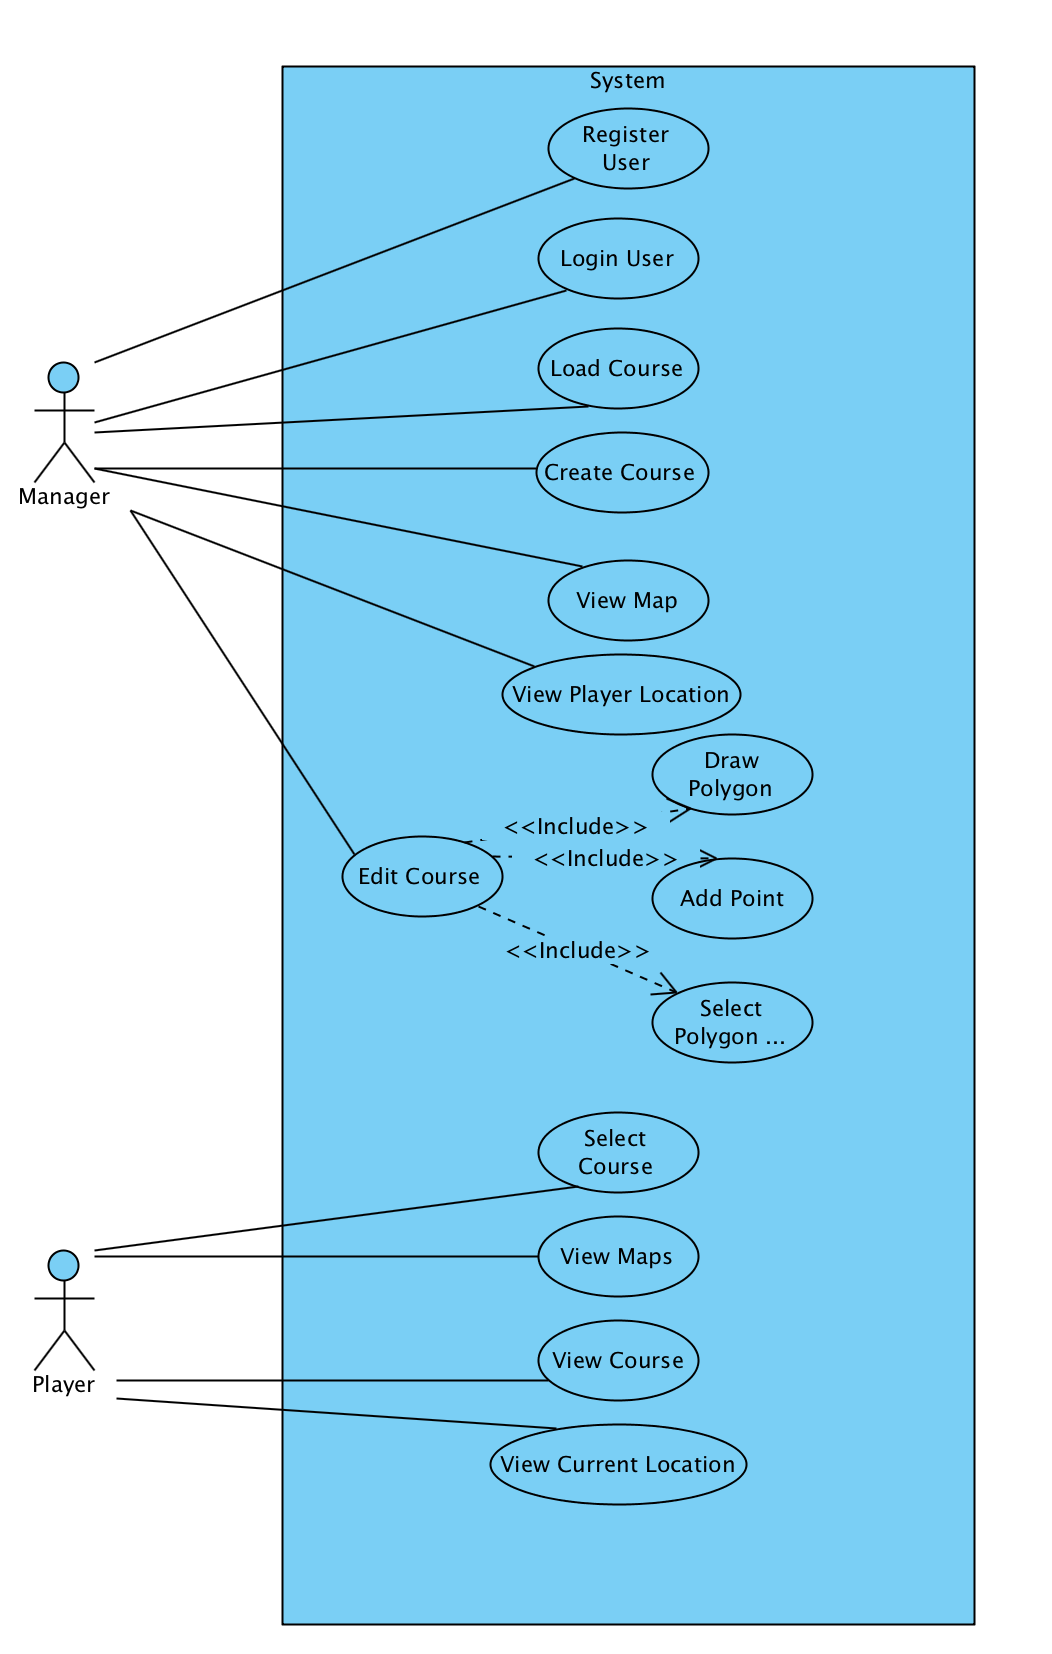
\includegraphics[scale=0.6]{UsecaseDiagram}
    \caption{Use case Diagram}
    \label{fig:usecase1}
    \end{figure}

    \subsection{Performance Requirements}
    \begin{itemize}
        \item
            The system shall be responsive.
        \item
            The system shall use the Google Maps API sparingly to reduce run
            cost.
    \end{itemize}

    \subsection{Architectural Requirements \& Design}

    \paragraph{}
    The System consists of three subsystems, namely the \textit{Mobile App}, the
    \textit{Website} and the \textit{Back End}. The Back End additionally
    consists of the \textit{DBMS} and \textit{API} subsystems. The system is
    designed according to the MVC (Model-View-Controller) architectural pattern.
    This choice is due to the fact that there is a single database that stores
    information about the golf courses and that there is more than one type of
    subsystem that interfaces with users. This allows the MVC pattern to be a
    good choice since it allows the abstraction of a model from the views, and
    also protects access to the model by the use of a controller. The
    abstraction created by the controller also increases the ease of maintaining
    the connection between the views and the model.

    \paragraph{}
    Figure \ref{deploymentdiagram} shows the deployment diagram of the system and it's
    subsystems. From here it is easy to identify the different components of the
    MVC pattern:

    \begin{itemize}
        \item \textbf{Model} - The DBMS serves as the model component by storing
            the information required by the system. The DBMS is solely and
            exclusively responsible for the store and retrieval of data,
            as well as enforcing integrity rules on the dataset.
        \item \textbf{Views} - The Mobile App and Website both serve as two
            different views. The Website is a view that uses the controller
            to both create, update and destroy data stored within the model
            in order to manage the mapping of golf courses. The Mobile App is
            a simpler view with the sole purpose of fetching and displaying
            data received from the model via the controller.
        \item \textbf{Controller} - The API serves as the controller. It acts
            as a level of abstraction between the model and the views by
            controlling the access to the model.
    \end{itemize}

    \paragraph{}

    \begin{center}
        \begin{figure}[h]
            \centering
            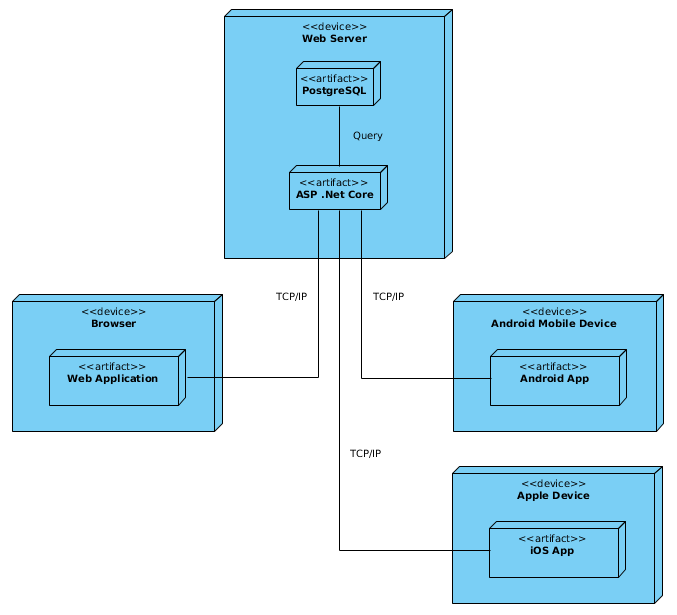
\includegraphics[scale=0.9]{DeploymentDiagram}
            \caption{Deployment diagram}
            \label{deploymentdiagram}
        \end{figure}
    \end{center}

\end{document}
